\chapter{Onde piane}
Le onde piane sono particolari soluzioni delle equazioni di Maxwell che hanno proprietà e simmetrie notevoli che ne semplificano notevolmente lo studio rispetto al caso generale.

\section{Equazioni di Helmholtz}
	Le equazioni di Maxwell possono essere riscritte come le cosiddette equazioni di Helmholtz, nel caso in cui il mezzo sia il vuoto.

	\begin{equation*}
		\begin{cases}
			\rot\E = - \jmath \, \omega \, \mu \, \H \\
			\rot\H = \jmath \, \omega \, \epsilon_c \, \E \\
		\end{cases}
	\end{equation*}

	Applicando, per esempio alla prima, l'operazione di rotore ad ambo i membri, e sostituendo la seconda si ottiene
	\begin{equation*}
		\begin{split}
			\rot\rot\E &= - \jmath \, \omega \, \mu \, \rot \rot\H \\
			- \nabla^2\E &= - \jmath \, \omega \, \mu \, (\jmath \, \omega \, \epsilon_c \, \E)\\
		\end{split}
	\end{equation*}

	\begin{equation} \label{eq:helmotz}
		\begin{cases}
			\nabla^2 \E + \omega^2 \, \mu \, \epsilon_c \, \E = 0 \\
			\nabla^2 \H + \omega^2 \, \mu \, \epsilon_c \, \H = 0
		\end{cases}
	\end{equation}

	Esse sono affini alle ben note equazioni delle onde: la loro soluzione sarà perciò nella forma

	\begin{equation} \label{eq:helmotz_sol}
		\begin{cases}
			E_x(\r) = E_{_{0}x} ~ e^{-\s \cdot \r} \\
			E_y(\r) = E_{_{0}y} ~ e^{-\s \cdot \r} \\
			E_z(\r) = E_{_{0}z} ~ e^{-\s \cdot \r}
		\end{cases}
	\end{equation}
	dove $\r$ è il vettore reale che definisce la posizione del punto considerato, mentre $\s = (s_x, s_y, s_z)$ è detto vettore \emph{di spostamento} e definisce come il campo vari nello spazio in modulo e fase.

	Sostituendo questa generica soluzione in \eqref{eq:helmotz}, si ottiene la condizione che il parametro $\s$ deve soddisfare per essere un'effettiva soluzione.

	\begin{equation} \label{eq:condizione_s}
		\begin{split}
			& \nabla^2 E_x+ \omega^2 \, \mu \, \epsilon_c \, E_x = 0 \\
			& E_{_0 x} ~ ({s_x}^2 e^{-\s \cdot \r} +
				{s_y}^2 e^{-\s \cdot \r} +
				{s_z}^2 e^{-\s \cdot \r}) +
				\omega^2 \, \mu \, \epsilon_c \, E_{_{0}x} ~ e^{-\s \cdot \r} = 0 \\
			& \s \cdot \s = {s_x}^2 + {s_y}^2 + {s_z}^2 = - \omega^2 \, \mu \, \epsilon_c
		\end{split}
	\end{equation}
	dove nell'ultimo passaggio la somma dei quadrati delle componenti di $\s$ è indicata, con un abuso di notazione, come il prodotto scalare \emph{reale} nonstante $\s$ sia un vettore complesso.

	Una volta individuate le condizioni per la validità della soluzione \eqref{eq:helmotz_sol}, si può stabilire il legame tra campo elettrico e magnetico.

	\begin{equation*}
		\begin{split}
			\H & = \frac {\rot\E}{- \jmath \omega \mu} =
				\frac {\rot(\vec{E_{_{0}}} ~ e^{-\s \cdot \r})}{- \jmath \omega \mu} \stackrel{(1)}{=} \\
			& = \frac {(\rot\vec{E_{_{0}}}) ~ e^{-\s \cdot \r} - \vec{E_{_{0}}} \times \nabla e^{-\s \cdot \r}} {- \jmath \omega \mu} \stackrel{(2)}{=} \\
			& = \frac{ \vec{E_{_{0}}} \times ( \s ~ e^{-\s \cdot \r})} {- \jmath \omega \mu} = \frac { \s \times \vec{E_{_{0}}}} {\jmath \omega \mu}
			~ e^{-\s \cdot \r} = \frac{\s \times \E}{\jmath \omega \mu} \\
		\end{split}
	\end{equation*}
	dove (1) è dato dalla derivata del prodotto, mentre (2) è dovuto al fatto che, essendo $\vec{E_{_{0}}}$ costante, il suo gradiente è nullo.

\section{Piani di simmetria}
	La soluzione di onda piana presenta particolari comportamenti lungo e trasversalmente le direzioni date dalla parte reale e immaginaria del vettore $\s = \a + \jmath \k$.

	\begin{itemize}
		\item[$\Delta\r \perp \a$ )] Lungo questa direzione, l'ampiezza dei campi $\E$ e $\H$ non cambia.

		\begin{equation*}
			\begin{split}
				|\E(\r + \Delta\r)| &= |\vec{E_{_{0}}}| ~ e^{-\a \cdot (\r + \Delta\r)} = \\
				& = |\vec{E_{_{0}}}| ~ e^{-\a \cdot \r} ~ e^{-\a \cdot \Delta\r} \stackrel{(*)}{=} \\
				& = |\vec{E_{_{0}}}| ~ e^{-\a \cdot \r} = |\E(\r)|
			\end{split}
		\end{equation*}
		dove (*) è dato dal fatto che $\a \cdot \Delta\r = 0$ per costruzione.

		\item[$\Delta\r \perp \k$ )] Lungo questa direzione, la fase dei campi $\E$ e $\H$ non cambia.

		\begin{equation*}
				\measuredangle \E(\r + \Delta\r) = -\k \cdot (\r + \Delta\r) \stackrel{(*)}{=} - \k \cdot \r = \measuredangle \E(\r)
		\end{equation*}
		dove (*) è dato dal fatto che $\k \cdot \Delta\r = 0$ per costruzione.

		\item[$\Delta\r \parallel \a$ )] Lungo questa direzione, l'ampiezza dei campi cala in modo esponenziale in $|\a|$ e in $\Delta r$.

		\begin{equation*}
			\begin{split}
				|\E(\r + \Delta\r)| &= |\vec{E_{_{0}}}| ~ e^{-\a \cdot (\r + \Delta\r)} = \\
				& = |\vec{E_{_{0}}}| ~ e^{-\a \cdot \r} ~ e^{-\a \cdot \Delta\r} \stackrel{(*)}{=} \\
				& = \left( |\vec{E_{_{0}}}| ~ e^{-|\a| \Delta\r} \right) e^{-\a \cdot \r} = |\E(\r)| ~ e^{-|\a| \Delta\r}
			\end{split}
		\end{equation*}
		dove (*) è dovuto al parallelismo tra $\a$ e $\Delta\r$.

		\item[$\Delta\r \parallel \k$ )] Lungo questa direzione, la fase dei campi $\E$ e $\H$ oscilla periodicamente.

		\begin{equation*}
				\measuredangle \E(\r + \Delta\r) = -\k \cdot (\r + \Delta\r) \stackrel{(*)}{=} - \k \cdot \r - |\k| \Delta r = \measuredangle \E(\r) - |\k| \Delta r
		\end{equation*}
		dove (*) è dovuto al parallelismo tra $\k$ e $\Delta\r$.

		Come si può osservare da questa periodicità della fase, i piano cosiddetti equifase sono separati da una distanza $\lambda$ funzione di $|\k| \stackrel{.}{=} \beta$.

		\begin{equation} \label{eq:lunghezza_donda}
			\lambda = \frac{2 \pi}{|\k|} = \frac{2 \pi}{\beta} \text{ è definita come \emph{lunghezza d'onda}}
		\end{equation}
	\end{itemize}

\section{Onda piana nel vuoto}
	Studieremo qui la propagazione dell'onda piana in un mezzo che, come il vuoto, è un perfetto isolante, ovvero $\sigma = 0$.

	Scomponendo l'equazione \eqref{eq:condizione_s}, si può ottenere il seguente sistema

	\begin{equation} \label{eq:s_components}
		\begin{dcases}
			& |\a|^2 - |\k|^2 = - \omega^2 \, \mu \, \epsilon \\
			& 2 \a \cdot \k = \omega \, \mu \, \sigma = 0
		\end{dcases}
	\end{equation}

	La seconda equazione è risolta per ciascuno dei seguenti casi
	\begin{equation}\begin{dcases}
		|\a| = 0 \\
		|\k| = 0 \\
		\a \perp \k
	\end{dcases}\end{equation}

	Il caso $|\k| = 0$ è da escludere a priori, perché la prima equazione del sistema \eqref{eq:s_components} diventa impossibile.

	\subsection{Onda piana uniforme}
		Concentriamoci sul caso $|\a| = 0$: esso porta alla soluzione cosiddetta di onda piana uniforme, che si propaga nel vuoto senza perdite di potenza.

		\begin{equation*}
				\a = 0 \implies |\k| = \sqrt{\omega^2 \mu \epsilon} = \omega \sqrt{\mu \epsilon} = \frac{\omega}{c} = \frac{2 \pi}{\lambda} = \beta
		\end{equation*}
		dove $c$ è la velocità della luce nel mezzo.

		Nei mezzi dielettrici $c$ è calcolabile come
		\begin{equation*}
				c = \frac{1}{\sqrt{\epsilon \mu_0}} = \frac{1}{\sqrt{\epsilon_0 \mu_0 \epsilon_r}} = \frac{c_0}{\sqrt{\epsilon_r}} = \frac{c_0}{n}
		\end{equation*}
		dove $n$ è definito come il coefficiente di rifrazione nel mezzo e $c_0$ è la velocità della luce nel vuoto.

	\subsection{Onda piana uniforme in polarizzazione rettilinea}
		Considerando il caso specifico di polarizzazione rettilinea, con $\vec{E_{_{0}}} = E_{_{0}} \, \hat{x}$, otteniamo che

		\begin{equation*} \begin{split}
			\vec{H_{_{0}}} &= \frac{\s \times \vec{E}} {\jmath \omega \mu}
				= \frac{(\jmath \k) \times (E_{_{0}} \, \hat{x})}{\jmath \omega \mu}
				= \frac{|\k| \, E_{_{0}}}{\omega \mu} ~ \hat{k} \times \hat{x} = \\
			& = \frac{|\k| \, E_{_{0}}}{\omega \mu} ~ \hat{y}
				= \frac{E_{_{0}}}{\mu c} ~ \hat{y}
				= \frac{E_{_{0}}}{\sqrt{\mu / \epsilon}} ~ \hat{y}
				= \frac{E_{_{0}}}{\eta} ~ \hat{y}
				= H_{_{0}} ~ \hat{y}
		\end{split} \end{equation*}
		dove $\eta$ è definita come impedenza d'onda del mezzo.

\section{Onda piana nel mezzo conduttore}
	Per i mezzi conduttori vale $\sigma \neq 0$, quindi si avrà il prodotto scalare $\a \cdot \k \neq 0$: questo rende impossibile il caso considerato in precedenza di onda piana uniforme, perché la componente reale di attenuazione (come pure il vettore $\k$) è sempre presente.

	\subsection{Onda piana nel buon conduttore} \label{sec:onda_piana_conduttore}
		Dividendo tra loro membro a membro le due equazioni del sistema \eqref{eq:s_components} si ottiene che

		\begin{equation*} \begin{split}
			& \frac{|\k|^2 - |\a|^2}{2 |\a| |\k| \cos(\theta)}
				= \frac{\omega^2 \mu \epsilon}{\omega \mu \sigma}
				= \frac{\omega \epsilon}{\sigma} \stackrel{(*)}{\ll} 1
		\end{split} \end{equation*}
		dove $\theta$ è l'angolo tra $\a$ e $\k$ e la disuguaglianza (*) è data dalla proprietà caratteristica dei buoni conduttori.

		Riformulando l'equazione sopra si ottiene che
		\begin{equation*}
			\frac{|\k|^2 - |\a|^2}{|\a| |\k|}
				= \frac{|\k|}{|\a|} - \frac{|\a|}{|\k|}
				\ll 2 \cos(\theta) < 2 \implies
				\begin{dcases}
					~ |\k| \simeq |\a| \\
					~ \k \parallel \a
				\end{dcases}
		\end{equation*}
		dove il passaggio al sistema di destra non è rigoroso, ma vuole presentare l'intuizione sottostante.

		Questa uguaglianza tra i due vettori $\a$ e $\k$ si può sfruttare per risolvere il sistema \eqref{eq:s_components}.
		\begin{equation*}
			\begin{dcases}
				~ |\k| \simeq |\a|
					= \sqrt{\frac{\omega \mu \sigma}{2}}
					= \sqrt{\pi f \mu \sigma} \\
				~ \s = (1 + \jmath) ~ \sqrt{\pi f \mu \sigma} ~ \hat{z} \\
			\end{dcases}
		\end{equation*}

		Un'onda polarizzata linearmente con questo valore di $\s$ avrà perciò campi
		\begin{equation*}
			\begin{dcases}
				~ \E = \vec{E_{_{0}}} ~ e^{-\s \cdot \r} = E_{_{0}} \hat{x} ~ e^{-|\a| (1 + \jmath) z} \\
				~ \H = \frac{\s \times \vec{E_{_{0}}}}{\jmath \omega \mu} ~ e^{-\s \cdot \r}
					= \ldots = \frac{E_{_{0}} |\a| (1 + \jmath)}{\jmath \omega \mu} ~ e^{-|\a| (1 + \jmath) z} ~ \hat{y}
					= \frac{E_{_{0}}}{ R_s (1 + \jmath) } ~ e^{-|\a| (1 + \jmath) z} ~ \hat{y}
			\end{dcases}
		\end{equation*}
		dove $R_s = \sqrt{\frac{\pi f \mu}{\sigma}}$ è la resistenza superficiale del mezzo e $Z_w = (1 + \jmath) R_s$ è l'impedenza di parete del mezzo.

		\subsubsection{Spessore di penetrazione}
		Nello studio della propagazione di onde in un mezzo, si definisce il cosiddetto \emph{spessore di penetrazione} come la distanza $\delta$ lungo l'asse di propagazione per cui il modulo del campo cala di un fattore $e^{-1}$.

		\begin{equation*}
			|\E(z + \delta)| = |\E(z)| ~ e^{-1}
		\end{equation*}

		Nel buon conduttore essa è facilmente calcolabile con le equazioni trovate in precedenza.
		\begin{equation} \begin{split} \label{eq:spessore_penetrazione}
			|\E(z + \delta)| = E_{_{0}} ~ e^{-|\a| z} ~ e^{-|\a| \delta} = |\E(z)| ~ e^{-|\a| \delta} = e^{-1} \text{ per } \delta = \frac{1}{|\a|}
		\end{split} \end{equation}

		Nel caso, per esempio del rame, $\delta$ risulta dell'ordine di $1.6 \mathrm{\mu m}$: questo ci porta a concludere che l'onda incidente il buon conduttore viene in gran parte dispersa vicino alla superficie del mezzo.
		Questo comportamento, dovuto in gran parte all'effetto Joule, viene chiamato \emph{effetto pelle}.

		Questo comportamento, dovuto principalmente all'effetto Joule, viene chiamato \emph{effetto pelle}.
		\subsubsection{Lunghezza d'onda nel buon conduttore}
		Il buon conduttore modifica le proprietà dell'onda che lo attraversa: riduce infatti notevolmente la sua lunghezza rispetto alla propagazione libera nel vuoto.
		\begin{equation*} \begin{split}
			& |\k|
				= \sqrt{\pi f \mu \sigma}
				\gg \omega \sqrt{\mu \epsilon}
				= |\vec{k_{_{0}}}| \\
		\end{split} \end{equation*}

		perché, per le proprietà del buon conduttore,
		\begin{equation*} \begin{split}
				\sqrt{\pi f \mu \sigma} &\gg \omega \sqrt{\mu \epsilon} \\
				2 \pi f \sigma &\gg 2 \omega^2 \epsilon \\
				\sigma &\gg 2 \omega \epsilon
		\end{split} \end{equation*}

		Da questo risultato e dalla definizione di $\lambda$ (equazione \eqref{eq:lunghezza_donda}) si ottiene quanto anticipato in precedenza, ovvero che
		\begin{equation*} \begin{split}
			& \lambda = \frac{2\pi}{|\k|} \ll \frac{2\pi}{|\vec{k_{_{0}}}|} = \lambda_{_{0}} \\
		\end{split} \end{equation*}

\section{Appendice sui vettori di \emph{Steimetz}}
	Dati due vettori complessi tridimensionali $\vec{A}, \vec{B} \in \mathbb{C}^3$, il prodotto scalare è definito come $\langle \vec{A} | \vec{B} \rangle = \vec{A} \cdot \vec{B}^* = \sum_{n=1}^3 A_n {B_n}^*$.

	Cerchiamo ora di stabilire cosa significhi, partendo dalla sua definizione,  l'ortogonalità tra due vettori complessi. Considereremo in particolare vettori che esprimano componenti lungo due soli assi, ovvero giacenti sul piano di polarizzazione.

	\begin{esp}
		& \vec{A} \perp \vec{B} \Leftrightarrow \vec{A} \cdot \vec{B}^* = 0 \quad \text{con}\quad \begin{dcases}
			\vec{A} = A_{x^{\prime}} \, \hat{x}^{\prime} + A_{y^{\prime}} \, \hat{y}^{\prime} \\
			\vec{B} = B_{x^{\prime}} \, \hat{x}^{\prime} + B_{y^{\prime}} \, \hat{y}^{\prime}
		\end{dcases}
	\end{esp}

	Risolvendo l'equazione, si dimostra che l'ortogonalità di vettori di questo tipo consiste in una particolare simmetria dei rapporti di polarizzazione.
	\begin{esp}
		&A_{x^{\prime}} \, B_{x^{\prime}}^* + A_{y^{\prime}} \, B_{y^{\prime}}^* = 0 \\
		&p_A^{\prime} = \jmath \frac{ A_{x^{\prime}} } { A_{y^{\prime}} }
			= - \jmath \frac{ B_{y^{\prime}} } { B_{x^{\prime}} }
			= \frac{1} {\jmath \frac{ B_{x^{\prime}}^* } { B_{y^{\prime}}^* }} = \frac{1}{ \left( -p_B^{\prime} \right)^* }
	\end{esp}

\section{Potenza dell'onda elettromagnetica}
	Partendo dalle ben note equazioni di Maxwell è possibile ottenere un bilancio energetico a cui le onde elettromagnetica devono sottostare.

	\begin{esp}
		\begin{dcases}
			\rot \e = - \mu \deriv{\h}{t} \\
			\rot \h = \jt + \sigma \e + \epsilon \deriv{\e}{t} \\
		\end{dcases}
	\end{esp}

	Combinando tra loro le equazioni, si ottiene che
	\begin{esp}
		& \rot \h \cdot \e - \h \cdot \rot \e
			= \e \cdot \j + \sigma |\e|^2 + \epsilon\, \e \deriv{\e}{t} + \h \mu \deriv{\h}{t} \\
		& -\diverg(\e \times \h) - \e \cdot \jt = \sigma |\e|^2 + \epsilon \deriv{|\e|^2}{t} + \mu \deriv{|\h|^2}{t}
	\end{esp}
	dove il primo membro è riscritto come divergenza grazie ad un'identità vettoriale.

	L'analisi dimensionale mette in luce come le quantità dell'equazione ricavata siano potenze per unità di volume: integrando sul volume $V$ considerato si ottengono perciò potenze, qui scomposte a seconda dell'origine dei vari termini.

	\begin{esp} \hspace*{-1cm}
		 \label{eq:bilancio_potenza_EM}
		& \underbrace{ - \int_V \e \cdot \jt dV}_{\text{potenza dai generatori}}
			= \underbrace{\int_V \sigma |\e|^2 dV}_{\text{effetto Joule}}
			+ \underbrace{\int_V \left[ \epsilon \deriv{|\e|^2}{t} + \mu \deriv{|\h|^2}{t} \right] dV}
				_{\text{variazione di energia \textsc{EM} in } V}
			+ \underbrace{\int_V \diverg(\e \times \h) dV}_{\text{flusso di potenza in uscita da }V} \\
		%& - \int_V \e \cdot \jt dV
		%	= \int_V \sigma |\e|^2 dV
		%	+ \deriv{}{t} \int_V \left[ \frac{\epsilon}{2} |\e|^2 - \frac{\mu}{2} |\h|^2 \right] dV
		%	+ \int_{S_V} (\e \times \h) \cdot \hat{n} ~ dV \\
	\end{esp}
	\subsection{Potenza espressa con vettori di Steinmetz}
	Cercheremo ora la relazione tra $|\ert|$ e il suo vettore associato $|\E|$, per stabilire come calcolare la potenza del campo oscillante $\e$ con il vettore di Steinmetz.

	\begin{esp}
		|\ert|^2
			& = \Re\left[ \E ~ e^{j \omega t}\right] \left( \Re\left[ \E ~ e^{j \omega t}\right] \right)^* \\
			& \stackrel{(1)}{=} \left( \frac{\E ~ e^{j \omega t} + \E ~ e^{-j \omega t}}{2} \right) ^2 \\
			& = \frac{1}{4} \left( \E \cdot \E^* +  \E^* \cdot \E + \E \cdot \E ~ e^{j 2 \omega t} + \E^* \cdot \E^* ~ e^{-j 2 \omega t} \right) \\
			& = \frac{|\E|^2}{2} +
				\frac{
					\E \cdot \E ~ e^{j 2 \omega t} +
					\E^* \cdot \E^* ~ e^{-j 2 \omega t}
				}{4}
	\end{esp}
	dove (1) deriva dall'uguaglianza $\Re[z] = \frac{z+z^*}{2}$
	Mediando nel periodo $T$ il modulo del quadrato del campo otteniamo la potenza del campo elettrico.

	\begin{esp}
		\frac{1}{T} \int_0^T |\ert|^2 dt
			& = \frac{1}{T} \int_0^T \frac{|\E|^2}{2} dt +
				\frac{1}{T} \int_0^T \left(
					\frac{
						\E \cdot \E ~ e^{j 2 \omega t} +
						\E^* \cdot \E^* ~ e^{-j 2 \omega t}
				}{4}\right) dt \\
			& \stackrel{(1)}{=}  \frac{1}{T} \int_0^T \frac{|\E|^2}{2} dt
				\stackrel{(2)}{=} \frac{|\E|^2}{2}
	\end{esp}
	dove (1) vale perché il secondo membro è periodico, perciò l'integrale sul periodo $T$ è nullo, mentre (2) è immediato perché il vettore $\E$ non dipende dal tempo $t$.

	Grazie alla relazione appena ricavata, è possibile applicare la trasformata di Steinmetz all'equazione \eqref{eq:bilancio_potenza_EM}, ottenendone il duale.

	\begin{esp} \label{eq:bilancio_potenza_EM_steinmetz}
		& \underbrace{ - \int_V \E \cdot \J^* ~ dV}_{\text{potenza dai generatori}}
			= \underbrace{\int_V \sigma \frac{|\E|^2}{2} dV}_{\text{effetto Joule}}
			+ \underbrace{\int_V \frac{\jmath \omega}{2} \left[\mu \frac{|\H|^2}{2} - \epsilon \frac{|\E|^2}{2} \right] dV}
				_{\text{variazione di energia \textsc{EM} in } V}
			+ \underbrace{ \int_V \frac{\diverg(\E \times \H^*)}{2} dV}_{\text{flusso di potenza in uscita da }V}
	\end{esp}

	\subsection{Vettore di Poynting}

	L'ultimo termine dell'equazione \eqref{eq:bilancio_potenza_EM_steinmetz} rappresenta la potenza trasportata dall'onda fuori dal volume $V$: esso è perciò di particolare interesse per il nostro studio.

	\begin{esp} \label{eq:def_poynting}
		\int_V \frac{\diverg(\E \times \H^*)}{2} dV
			= \int_{S_V} \frac{\E \times \H^*}{2} \cdot \hat{n} ~ dS
			= \int_{S_V} \vec{P} \cdot \hat{n} ~ dS
	\end{esp}
	dove $\vec{P}$ è chiamato \emph{vettore di Poynting}, e individua il verso della trasmissione di potenza portata dall'onda attraverso $S_V$.

	Da ciò, l'intensità dell'onda viene definita a partire dal vettore $\vec{P}$, come
	\begin{equation}
		I = \Re[\vec{P}]
	\end{equation}


	\subsubsection{Poynting per l'onda piana nel vuoto}

		Nel caso dell'onda piana su un perfetto isolante, si ha che la parte reale del bilancio di potenze \eqref{eq:bilancio_potenza_EM_steinmetz} si semplifica notevolmente.

		\begin{esp} \label{eq:bilancio_potenza_EM_steinmetz}
			& \underbrace{ - \int_V \frac{\E \cdot \J}{2} ~ dV}_{= 0 \text{ perché } \jt = 0}
				= \underbrace{\int_V \sigma \frac{|\E|^2}{2} dV}_{= 0 \text{ perché } \sigma = 0}
				+ \int_{S_V} \Re[\vec{P}] \cdot \hat{n} ~ dS
				\implies \int_{S_V} \Re[\vec{P}] \cdot \hat{n} ~ dS = 0
		\end{esp}

		Da qui emerge che in questo caso privo di sorgenti e di dispersioni, $\Re[\vec{P}]$ è un campo solenoidale.

		Nel caso ancora più specifico di polarizzazione rettilinea il vettore di Poynting si calcola semplicemente come
		\begin{esp}
			\vec{P}
				= \frac{1}{2} \left( E_{_{0}} \hat{x} \right) \times \left( \frac{E_{_{0}}}{\eta} \hat{y} \right)
					~ e^{\jmath \beta z} ~ e^{- \jmath \beta z}
				= \frac{|E_{_{0}}|^2}{2\eta} \hat{z}
				= I \hat{z}
		\end{esp}

		In questo caso possiamo osservare che
		\begin{equation}
			\begin{dcases}
				~ \vec{P} \in \mathbb{R}^3 & \text{ la potenza trasmessa è puramente reale} \\
				~ |\vec{P}| \propto |E_{_{0}}|^2 \\
				~ \vec{P} \parallel \hat{z}, \k & \text{ la potenza è trasmessa lungo l'asse } \hat{z}
			\end{dcases}
		\end{equation}

	\subsubsection{Poynting per l'onda piana nel buon conduttore}
		Analogamente rispetto al caso di onda piana nel vuoto, $\vec{P}$ si calcola a partire dalle espressioni per i campi $\E$ e $\H$.

		\begin{equation}
			\begin{dcases}
				~ \E = \vec{E_{_{0}}} \hat{x} ~ e^{-\beta(1+\jmath) z} \\
				~ \H = \vec{H_{_{0}}} \hat{x} ~ e^{-\beta(1+\jmath) z} \\
			\end{dcases}
			\text{ con } \beta = |\k| = |\a| = \sqrt{\pi f \sigma \mu}
		\end{equation}

		Applicando la definizione di vettore di Poynting si ha perciò

		\begin{esp}
			\vec{P} &
				= \frac{\E \times \H^*}{2} \\
			& = \frac{1}{2} \left( E_{_{0}} \hat{x} \right)
					\times \left( \frac{H_{_{0}}^*}{Z_w^*} \hat{y} \right)
					~ e^{-\beta(1+\jmath) z} ~ e^{-\beta(1-\jmath) z} \\
			& = \frac{|E_{_{0}}|^2}{2 Z_w*} \hat{z} ~ e^{-2 \beta z}
				= \frac{|E_{_{0}}|^2}{2 R_s (1 - \jmath)} \hat{z} ~ e^{-2 \beta z} \\
			& = \left( \frac{|E_{_{0}}|^2}{4 R_s} \hat{z} ~ e^{-2 \beta z} \right)  (1 + \jmath) \\
			& = \Re[\vec{P}]  (1 + \jmath)
		\end{esp}

		dove si può notare come l'intensità $I = \Re[\vec{P}] $ cali esponenzialmente in $z$, secondo $\beta = |\a|$.

		Dopo lo spessore di penetrazione $\delta$, definito nell'equazione \eqref{eq:spessore_penetrazione}, l'intensità risulta ridotta di un fattore $e^{-2} \simeq 1/9$, diventando così trascurabile per distanze superiori ai 3--5 $\delta$.

\section{Riflessione e rifrazione}
Riflessione e rifrazione sono trasformazioni a cui l'onda elettromagnetica è sottoposta quando attraversa la frontiera tra due materiali differenti, come in \autoref{fig:discontinuita}.

L' analisi consiste perciò nel risolvere le equazioni di Maxwell nei due mezzi e poi garantire la continuità delle soluzioni sulla superficie di separazione.

\def\height{3}
\def\length{6}

\begin{figure}[h]
	\centering
	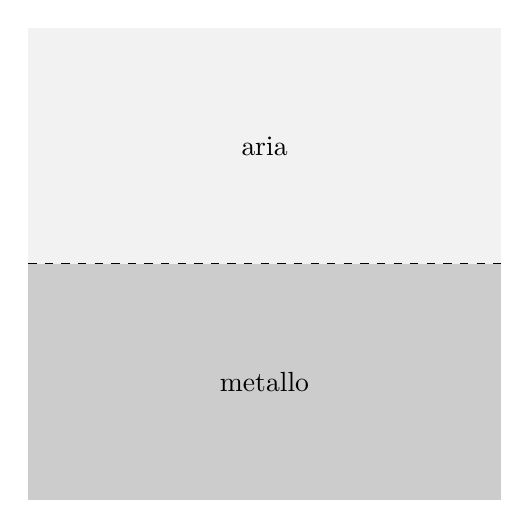
\begin{tikzpicture}
		\fill[black!20]
			(0, 0) rectangle
			(\length, \height)
			node [pos=0.5,text=black] {metallo};

		\fill[black!5]
			(0, \height) rectangle
			(\length, 2*\height)
			node [pos=0.5,text=black] {aria};

		\draw [dashed] (0, \height) -- (\length, \height);
	\end{tikzpicture}
	\caption{La discontinuità tra i materiali è evidenziata dalla linea tratteggiata.}
	\label{fig:discontinuita}
\end{figure}

\subsubsection{Continuità dei campi tangenti}
Un importante lemma permette di far coincidere le soluzioni sulla discontinuità: esso afferma che la componente dei campi $\E$ ed $\H$ tangente alla superficie resta costante nel passaggio tra il primo ed il secondo mezzo.

\begin{equation}
	\begin{dcases}
		~ \E_{1, tg} = \E_{2, tg} \\
		~ \H_{1, tg} = \H_{2, tg}
	\end{dcases}
\end{equation}

\subsection{Incidenza tra perfetti isolanti}
	Nel caso $\k \perp \hat{n}$, ovvero incidenza normale alla superficie e $\sigma_1 = \sigma_2 = 0$ si ha che, come rappresentato in \autoref{fig:incidenza_normale_isolanti}, la lunghezza d'onda si riduce: in particolare vale che

	\begin{esp}
		\begin{dcases}
			c_1 = \frac{c_{_{0}}}{n_1} \\
			c_2 = \frac{c_{_{0}}}{n_2}
		\end{dcases}
		\implies
		\begin{dcases}
			\lambda_1 = \frac{\lambda_{_{0}}}{n_1} \\
			\lambda_2 = \frac{\lambda_{_{0}}}{n_2}
		\end{dcases}
		\implies
		\lambda_2 = \lambda_1 \frac{n_1}{n_2}
	\end{esp}

	\begin{figure}[ht]
		\centering
		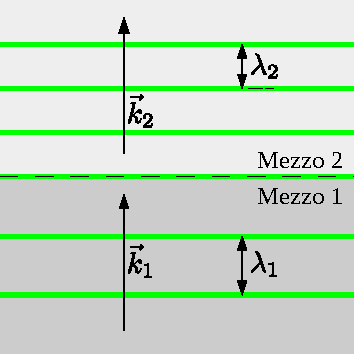
\includegraphics{img/incidenza_normale.pdf}
		\caption{I piani equifase, evidenziati in verde, riducono la distanza tra loro, ovvero la lunghezza d'onda $\lambda_2 < \lambda_1$ nel caso $n_2 > n_1$.}
		\label{fig:incidenza_normale_isolanti}
	\end{figure}

	Nel caso invece di incidenza con un angolo $\theta_i$ rispetto alla normale della superficie, il comportamento è più complesso, come si può osservare in \autoref{fig:incidenza_non_normale_isolanti}.

	La continuità dei piani equifase ci permette ancora di valutare il comportamento dell'onda anche senza risolvere le equazioni di Maxwell.

	Considerando il segmento $l$ evidenziato in figura, la sua lunghezza può essere calcolata in due modi diversi, grazie alle proprietà dei triangoli rettangoli.

	\begin{esp} \label{eq:legge_di_snell}
		l = \frac{\lambda_1}{\sin(\theta_i)} = \frac{\lambda_2}{\sin(\theta_t)}
	\end{esp}

	\begin{figure}[ht]
		\centering
		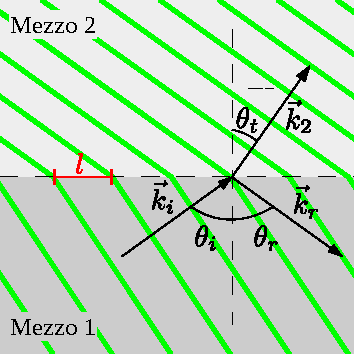
\includegraphics{img/incidenza_non_normale.pdf}
		\caption{La continuità dei campi tangenti impone che i piano equifase conservino la stessa distanza $l$ tra loro \emph{sulla superficie di separazione}.}
		\label{fig:incidenza_non_normale_isolanti}
	\end{figure}

	Nel caso i due elementi abbiamo lo stesso indice di rifrazione $n_i$, l'onda procede senza variazioni: per $\lambda_1 = \lambda_2$ vale infatti che $\theta_1 = \theta_2$.
	Possiamo osservare che questo è ciò che accade per l'onda riflessa, per la quale $\theta_i = \theta_r$, appunto perché l'onda non cambia materiale di propagazione.

\subsection{Coefficienti di riflessione e trasmissione}
	Nella sezione precedente abbiamo osservato come individuare le direzioni dell'onda riflessa e di quella trasmessa: ci focalizzaremo quindi su come la discontinuità influenzi il modulo del campo elettromagnetico.

	Per semplicità di calcolo e notazione ci metteremo nel caso di incidenza normale, ma analogamente segue per il caso generale.

	\begin{figure}[ht]
		\centering
		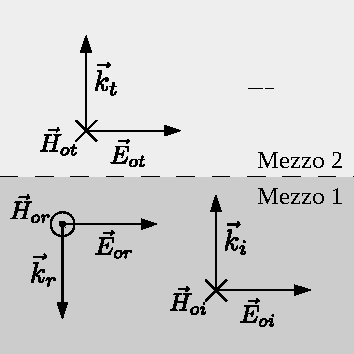
\includegraphics{img/campi_incidenza_normale.pdf}
		\caption{Nella riflessione il campo $\E$ mantiene la sua direzione, mentre $\H$ la inverte. Questo è dovuto ad un asimmetria delle equazioni di Maxwell legata al teorema delle immagini.}
		\label{fig:campi_incidenza_normale_isolanti}
	\end{figure}

	Nella superficie di discontinuità i campi sono tutti paralleli, quindi le somme vettoriali si riducono a somme scalari.
	\begin{esp}
		\begin{cases}
			E_{_0 i} + E_{_0 r} = E_{_0 t} \\
			H_{_0 i} - H_{_0 r} = H_{_0 t}
		\end{cases} \implies
		\frac{E_{_0 i}}{\eta_1} - \frac{E_{_0 r}}{\eta_1} = \frac{E_{_0 t}}{\eta_2} = \frac{E_{_0 i} + E_{_0 r}}{\eta_2}
	\end{esp}
	dove sono state impiegate le formule che legano $|\E|$ e $|\H|$ nel caso dell'onda piana.

	Riorganizzando i termini dell'equazione, si ottiene il \emph{coefficiente di riflessione} $\rho$.
	\begin{esp} \label{eq:coefficiente_riflessione}
		& \rho \stackrel{.}{=} \frac{E_{_0 r}}{E_{_0 i}}
			= \frac{\eta_2 - \eta_1}{\eta_2 + \eta_1}
			\stackrel{(*)}{=} \frac{ \frac{\eta_{_{0}}}{n_2} - \frac{\eta_{_{0}}}{n_1}}{\frac{\eta_{_{0}}}{n_2} + \frac{\eta_{_{0}}}{n_1}}
			= \frac{n_2 - n_1}{n_2 + n_1}
	\end{esp}
	dove (*) vale solamente per i dielettrici, materiali per cui $\eta_i = \frac{\eta_{_{0}}}{n_i}$.

	Il \emph{coefficiente di trasmissione} $\tau$ si può ricavare in modo analogo.
	\begin{esp}
		& \tau \stackrel{.}{=} \frac{E_{_0 t}}{E_{_0 i}}
				= \frac{E_{_0 r} + E_{_0 i}}{E_{_0 i}}
				= \frac{E_{_0 r}}{E_{_0 i}} + 1
				= \rho + 1 \\
	\end{esp}

\subsection{Potenza trasmessa e riflessa}
	A partire dai valori del campo elettrico trasmessi e riflessi è possibile calcolare come si distribuisca la potenza dell'onda nei due materiali.

	\begin{esp}
		I_t
		& = |\Re[\vec{P}]|
			= \frac{|E_{_0 t}|^2}{2 \eta_2}
			= \frac{|E_{_0 i} (1 + \rho)|^2}{2 \eta_2} \\
		& = \frac{|E_{_0 i}|^2}{2 \eta_1} \frac{\eta_1}{\eta_2} |1 + \rho|^2
			= I_i \frac{\eta_1}{\eta_2} |1 + \rho|^2 \\
		& = I_i \frac{4 \eta_1 \eta_2}{|\eta_1 + \eta_2|^2}
			= I_i (1 - |\rho|^2) = I_i - I_i |\rho|^2 = I_i - I_r
	\end{esp}

	È possibile osservare come tutto il comportamento in potenza sia dovuto al solo parametro $\rho$, che definisce sia l'intensità dell'onda trasmessa che quella riflessa.

\subsection{Interferenza in riflessione}
	Come è possibile notare in \autoref{fig:campi_incidenza_normale_isolanti}, nel secondo mezzo c'è un'unica onda che si propaga, mentre nel primo ce ne sono due.
	Questo dà vita a fenomeni di interferenza tra l'onda progressiva incidente e l'onda regressiva riflessa generata dalla discontinuità di mezzo.

	\begin{figure}[ht]
		\centering
		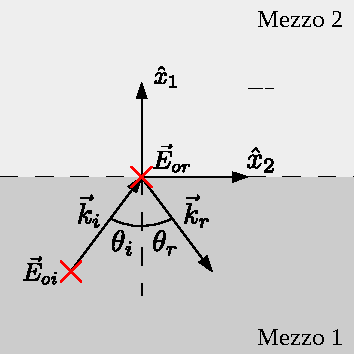
\includegraphics{img/campi_incidenza_non_normale.pdf}
		 \caption{Per l'onda considerata, i campi elettrici sono evidenziati per renderli più visibili e risultano paralleli all'asse $\hat{x}_3$ entrante nel foglio.}
		\label{fig:campi_incidenza_non_normale_isolanti}
	\end{figure}

	Nel caso generico di incidenza, abbiamo che
	\begin{esp}
		\begin{dcases}
			\k_i = (+ \beta_1 \cos(\theta_1), + \beta_1 \sin(\theta_1), 0) \\
			\k_r = (- \beta_1 \cos(\theta_1), + \beta_1 \sin(\theta_1), 0)
		\end{dcases}
	\end{esp}
	dove i vettori sono scomposti nelle loro componenti secondo il sistema di coordinate in \autoref{fig:campi_incidenza_non_normale_isolanti}.

	Il campo nel mezzo 1 si può perciò scrivere come
	\begin{esp}
		\E_1(\r)
		& = \E_{_0 i} ~ e^{-\jmath \k_i \cdot \r} + \E_{_0 r} ~ e^{-j \k_r \cdot \r} \\
		& = E_{_0 i} ~ \hat{x}_3
			~ e^{-\jmath \beta_1 [ \cos(\theta_i) \, x_1 + \sin(\theta_i) \, x_2] }
			+ E_{_0 r} ~ \hat{x}_3
			~ e^{-\jmath \beta_1 [-\cos(\theta_i) \, x_1 + \sin(\theta_i) \, x_2] } \\
		& = E_{_0 i} ~ \hat{x}_3
			~ e^{-\jmath \beta_1 [ \cos(\theta_i) x_1 + \sin(\theta_i) x_2] }
			+ E_{_0 i} (1 + \rho)
			~ \hat{x}_3 ~ e^{-\jmath \beta_1 [-\cos(\theta_i) x_1 + \sin(\theta_i) x_2]} \\
		& = E_{_0 i} (1 + \rho ~ e^{\jmath 2 \beta_1 \cos(\theta_i) x_1} )
			~ e^{-\jmath \beta_1 [\cos(\theta_i) x_1 + \sin(\theta_i) x_2]} \\
	\end{esp}

	Il modulo quadro del campo elettrico oscilla in funzione della posizione $x_1$, alternando piani di interferenza distruttiva (campo nullo) a piani di interferenza costruttiva (campo massimo).

	In particolare, nel caso di incidenza normale si ha che
	\begin{esp}
		|\E_1(\r)|^2
			& = |E_{_0 i}|^2 |1 + \rho ~ e^{\jmath 2 \beta_1 x_1}|^2 \\
			& = |E_{_0 i}|^2
				(1 + \rho ~ e^{\jmath 2 \beta_1 x_1})
				(1 + \rho^* ~ e^{-\jmath 2 \beta_1 x_1}) \\
			& = |E_{_0 i}|^2 (1 + |\rho|^2 + 2 |\rho| \cos(2 \beta_1 x_1+\phi_{\rho})) \\
	\end{esp}

	Questi piani individuano lungo $\hat{x}_3$ settori in cui l'impedenza vista dall'onda elettromagnetica varia. Essa, nel caso dell'onda piana, può essere calcolata sfruttando la legge di Ohm.

	\begin{esp}
		Z(x_1)
		& = \frac{E(x_1)}{H(x_1)}
			= \frac
				{E_{_0 i} (1 - e^{\jmath 2 \beta_1 x_3}) ~ e^{- \jmath \beta_1 x_3}}
				{-\frac{E_{_0 i}}{\eta_1} (1 + e^{\jmath 2 \beta_1 x_3}) ~ e^{- \jmath \beta_1 x_3} } \\
		& = \eta_1 ~ \frac
			{e^{\jmath \beta_1 x_3} - e^{\jmath \beta_1 x_3}}
			{e^{\jmath \beta_1 x_3} + e^{\jmath \beta_1 x_3}} \\
		& = \frac{\eta_1}{\jmath} ~ \frac{\sin(\beta_1 x_3)}{\cos(\beta_1 x_3)}
			= -\jmath \, \eta_1 \tan(\beta_1 x_3)
	\end{esp}

	Periodicamente ogni $\lambda_1 / 2$ l'impedenza d'onda oscilla da 0 a $+\infty$:

	\begin{esp}
		\forall m \in \mathbb{N}, ~
		\begin{dcases}
			Z \left( x_3 = -\frac{\lambda_1}{4} - m \frac{\lambda_1}{2} \right) = +\infty
				& \text{circuito aperto} \\
			Z \left( x_3 = - m \frac{\lambda_1}{2} \right) = 0
				& \text{perfetto conduttore} \\
		\end{dcases}
	\end{esp}

\subsection{Riflessione su un buon conduttore}
	Richiamando i risultati ottenuti nella sezione \ref{sec:onda_piana_conduttore}, se il mezzo di trasmissione (mezzo 2) è un buon coduttore, vale che

	\begin{esp}
		\begin{cases}
			|\a| \simeq |\k| = \sqrt{\pi f \mu_{_{0}} \sigma} \\
			\lambda_2 \ll \lambda_1
		\end{cases}
	\end{esp}

	La legge di Snell, dimostrata in precedenza nell'equazione \eqref{eq:legge_di_snell}, vale anche in questo caso, ed emerge che la trasmissione è sostanzialmente normale anche per angoli di incidenza diversi da $0^\circ$.

	\begin{esp}
		\sin(\theta_t)
			= \frac{\lambda_2}{\lambda_1} \sin(\theta_t)
			= \begin{cases}
				0 & \theta_i = 0 \\
				\sim 0 & \theta_i \simeq 0
			\end{cases}
			\text{\quad perché } \lambda_2 \ll \lambda_1
	\end{esp}

	Inoltre si può dimostrare come un buon conduttore si comporti come uno specchio per l'onda elettromagnetica, infatti, richiamando l'equazione \eqref{eq:coefficiente_riflessione}, si ha che

	\begin{esp}
		\rho
			= \frac{Z_w - \eta_1}{Z_w + \eta_1}
			= \frac{R_s (1 + \jmath) - \eta_1}{R_s (1 + \jmath) + \eta_1}
			\simeq -1
	\end{esp}
	dove l'ultimo passaggio è giustificato dal fatto che, per i buoni conduttori, la resistenza di parete $R_s$ è molto più piccola dell'impedenza del mezzo isolante $\eta_1$.

	Per esempio, nel passaggio dell'onda dall'aria al rame, si può calcolare che
	\begin{esp}
		\begin{cases}
			R_s = \sqrt{\frac{\pi f \mu_{_{0}}}{\sigma}} \simeq 60m\Omega \\
			\eta_1 = \frac{\eta_{_{0}}}{n_1} \simeq 377\Omega \gg R_s
		\end{cases}
	\end{esp}

	Con valore di $\rho$ come questo, si ha che $I_t = I_i (1 - |\rho|^2) \simeq 0$: il nostro materiale è un buono specchio e diventa uno specchio perfetto per $\sigma \to +\infty$.

%%% Local Variables:
%%% mode: latex
%%% TeX-master: "antenne"
%%% End:
